% Appendix C -- the full ablation suite. Ablations B and D keep their PH = 30
% tables in the body; their 60-minute halves and extended discussion are here.
\section{Comprehensive Ablation Studies}
\label{app:ablations}

\subsection{Ablation A: Does Multi-Task Coupling Help?}
\label{sec:ablation_a}

\begin{table*}[t]
\centering
\small
\setlength{\tabcolsep}{4pt}
\caption{Ablation A: multi-task coupling (PH = 30 min). Single-task arms zero the other task's loss weight, so the trunk is trained by one objective; the untrained head's metrics are reported but not meaningful. All ablation arms share one budget (20 epochs, fit split subsampled $2\times$), lighter than Table~\ref{tab:sota_ph30}'s (30 epochs, full fit split); rows here compare to each other, not to Table~\ref{tab:sota_ph30}.}
\label{tab:ablation_a_multitask_ph30}
\resizebox{\ifdim\width>\linewidth\linewidth\else\width\fi}{!}{%
\begin{tabular}{lrrrrrrrr}
\toprule
Arm & PR-AUC & ROC-AUC & Se@5\% & FAPD@5\% & Onset lead (min) & RMSE & Lag (min) & A+B (\%) \\
\midrule
Regression only & 0.028 & 0.3187 & 0.030 & 5.61 & 26.2 & \textbf{18.19} & \textbf{20.0} & 99.34 \\
Classification only & \textbf{0.868} & \textbf{0.9915} & \textbf{0.963} & 2.06 & \textbf{26.4} & 23.27 & 30.0 & 98.96 \\
Joint, fixed $\lambda=1$ & 0.842 & 0.9890 & 0.952 & 2.72 & 26.0 & 18.37 & 20.0 & \textbf{99.39} \\
Joint, Kendall uncertainty & 0.865 & 0.9912 & 0.959 & 2.87 & 26.4 & 18.49 & 20.0 & 99.36 \\
\bottomrule
\end{tabular}}
\end{table*}

\begin{table*}[t]
\centering
\small
\setlength{\tabcolsep}{4pt}
\caption{Ablation A: multi-task coupling (PH = 60 min). Single-task arms zero the other task's loss weight, so the trunk is trained by one objective; the untrained head's metrics are reported but not meaningful. All ablation arms share one budget (20 epochs, fit split subsampled $2\times$), lighter than Table~\ref{tab:sota_ph30}'s (30 epochs, full fit split); rows here compare to each other, not to Table~\ref{tab:sota_ph30}.}
\label{tab:ablation_a_multitask_ph60}
\resizebox{\ifdim\width>\linewidth\linewidth\else\width\fi}{!}{%
\begin{tabular}{lrrrrrrrr}
\toprule
Arm & PR-AUC & ROC-AUC & Se@5\% & FAPD@5\% & Onset lead (min) & RMSE & Lag (min) & A+B (\%) \\
\midrule
Regression only & 0.109 & 0.6749 & 0.143 & 4.77 & 41.2 & \textbf{30.84} & \textbf{40.0} & 97.73 \\
Classification only & \textbf{0.775} & \textbf{0.9728} & \textbf{0.856} & 2.37 & 42.7 & 38.13 & 60.0 & 96.91 \\
Joint, fixed $\lambda=1$ & 0.761 & 0.9703 & 0.840 & 3.29 & 43.5 & 31.29 & 40.0 & \textbf{97.93} \\
Joint, Kendall uncertainty & 0.772 & 0.9714 & 0.849 & 3.37 & \textbf{43.5} & 31.61 & 40.0 & 97.80 \\
\bottomrule
\end{tabular}}
\end{table*}


Single-task arms are obtained by zeroing the other task's loss weight, so the
four arms differ only in the objective; a gradient test confirms the silenced
head receives none, and its reported metrics are consequently meaningless.

Model selection follows each arm's own objective, and we state the monitors
explicitly because leaving them implicit would invite exactly the suspicion the
choice is meant to avoid. The regression-only arm is early-stopped on
\texttt{val/rmse} (minimised); the classification-only arm and both joint arms
are early-stopped on \texttt{val/pr\_auc} (maximised). Patience, maximum epochs,
optimiser, seed and every other budget parameter are identical across the four.
Using one monitor for all of them was the alternative and it is worse in both
directions: early-stopping the regression-only arm on PR-AUC would select on a
head that received no gradient, i.e.\ on noise, while early-stopping the
classification-only arm on RMSE would do the same in reverse. Each arm is
therefore stopped at its own best, which is the comparison that gives the
single-task specialists their strongest showing, which are the arms this study is
designed to be compared against unfavourably. The monitor is recorded in each arm's serialised
specification in the results JSON, so the choice is auditable rather than
asserted.

Joint training costs a little of each specialist. At $\PH = 30$ the
classification-only arm reaches PR-AUC $\NumAblAClsPRAUCHThirty$ and the joint
Kendall model $\NumAblAKendallPRAUCHThirty$, a cost of
$\NumAblAMultitaskCostHThirty$; the regression-only arm reaches RMSE
$\NumAblARegRMSEHThirty$ against the joint model's
$\NumAblAKendallRMSEHThirty$.

The comparison this study was designed to test, Kendall weighting against a fixed
$\lambda = 1$ (not tuned), does not resolve. Kendall weighting has the higher
PR-AUC, by $\NumAblAKendallEdgeHThirty$ at $\PH = 30$ and
$\NumAblAKendallEdgeHSixty$ at $\PH = 60$, and the fixed weight has the lower
RMSE at both horizons. Each is one run, and the differences are comparable to
the seed-to-seed range of the neural arms in the multi-seed benchmark. We therefore make
no accuracy claim for uncertainty weighting.

\paragraph{The case for the joint head is a deployment constraint, not an
accuracy claim.} We want to be explicit about this, because the ablation invites
the opposite reading: the specialists are not beaten, and a reader is right to
ask why the coupled model is preferred when a classification-only arm reaches
$\NumAblAClsPRAUCHThirty$ PR-AUC. The answer is that the target is an embedded
medical device, and on such a device the relevant comparison is not one joint
model against one specialist but one joint model against \emph{two} specialists
that must both be resident. A system that regresses glucose and forewarns
hypoglycemia needs both outputs at every five-minute tick; separating them means
shipping and maintaining two model binaries, two sets of weights in flash, two
inference sessions in a fixed RAM budget, two export-and-parity gates in the
release pipeline, and two artefacts to re-certify whenever either is retrained.
The trunk is where nearly all the parameters and nearly all the arithmetic live,
and the two tasks read the same physiology at the same lead times, so the
duplicated trunk serves no purpose.

Set against that, the measured price of coupling is
$\NumAblAMultitaskCostHThirty$ PR-AUC at $\PH = 30$ and a comparable margin on
RMSE ($\NumAblARegRMSEHThirty$ specialist against
$\NumAblAKendallRMSEHThirty$ joint). One trunk, four heads, one set of weights,
one conformal calibration and one $\NumEdgePFifty$~ms inference call
(Section~\ref{sec:edge}) deliver both outputs and their intervals for that
margin. Uncertainty weighting earns its place inside that design for a
maintenance reason rather than an accuracy one: the two losses live on
incompatible scales, so a fixed $\lambda$ is a hyperparameter that must be
re-tuned whenever the horizon set, the cohort or the class prior changes, and a
device pipeline is exactly where such a knob is most expensive to get wrong. We
present the multi-task head as Pareto-optimal under the deployment constraint,
not as a win on the accuracy axis the ablation measures. Had the coupling cost
been large rather than a few thousandths of PR-AUC, that argument would not have
been available.

\subsection{Ablation B: The Asymmetry Trade-Off}
\label{sec:appendix_ablation_b}

\begin{table*}[t]
\centering
\small
\setlength{\tabcolsep}{4pt}
\caption{Ablation B: asymmetric hypoglycemia cost (PH = 30 min). $\kappa$ multiplies the regression loss when the reference is hypoglycemic and the prediction sits above it; $\kappa = 1$ is a no-op. All ablation arms share one budget (20 epochs, fit split subsampled $2\times$), lighter than Table~\ref{tab:sota_ph30}'s (30 epochs, full fit split); rows here compare to each other, not to Table~\ref{tab:sota_ph30}.}
\label{tab:ablation_b_asymmetry_ph30}
\resizebox{\ifdim\width>\linewidth\linewidth\else\width\fi}{!}{%
\begin{tabular}{lrrrrrrr}
\toprule
Arm & RMSE & RMSE $<$70 & Bias $<$70 & D+E ($n$) & A+B (\%) & PR-AUC & Se@5\% \\
\midrule
$\kappa$ = 1 & \textbf{18.24} & 15.28 & +9.98 & 258 & 99.08 & \textbf{0.868} & \textbf{0.959} \\
$\kappa$ = 2 & 18.35 & 13.98 & +7.83 & 211 & 99.24 & 0.863 & 0.958 \\
$\kappa$ = 3 & 18.49 & 12.97 & +6.70 & 179 & 99.36 & 0.865 & 0.959 \\
$\kappa$ = 5 & 18.67 & 11.63 & +4.45 & 147 & 99.47 & 0.855 & 0.946 \\
$\kappa$ = 8 & 18.90 & \textbf{11.06} & +3.07 & \textbf{119} & \textbf{99.57} & 0.856 & 0.946 \\
\bottomrule
\end{tabular}}
\end{table*}

\begin{table*}[t]
\centering
\small
\setlength{\tabcolsep}{4pt}
\caption{Ablation B: asymmetric hypoglycemia cost (PH = 60 min). $\kappa$ multiplies the regression loss when the reference is hypoglycemic and the prediction sits above it; $\kappa = 1$ is a no-op. All ablation arms share one budget (20 epochs, fit split subsampled $2\times$), lighter than Table~\ref{tab:sota_ph30}'s (30 epochs, full fit split); rows here compare to each other, not to Table~\ref{tab:sota_ph30}.}
\label{tab:ablation_b_asymmetry_ph60}
\resizebox{\ifdim\width>\linewidth\linewidth\else\width\fi}{!}{%
\begin{tabular}{lrrrrrrr}
\toprule
Arm & RMSE & RMSE $<$70 & Bias $<$70 & D+E ($n$) & A+B (\%) & PR-AUC & Se@5\% \\
\midrule
$\kappa$ = 1 & \textbf{30.92} & 29.72 & +22.78 & 701 & 97.41 & \textbf{0.777} & \textbf{0.862} \\
$\kappa$ = 2 & 31.29 & 30.06 & +21.33 & 630 & 97.65 & 0.772 & 0.854 \\
$\kappa$ = 3 & 31.61 & 27.63 & +18.83 & 583 & 97.80 & 0.772 & 0.849 \\
$\kappa$ = 5 & 32.04 & 24.49 & +14.71 & 496 & 98.15 & 0.757 & 0.826 \\
$\kappa$ = 8 & 32.31 & \textbf{23.88} & +13.23 & \textbf{477} & \textbf{98.20} & 0.760 & 0.839 \\
\bottomrule
\end{tabular}}
\end{table*}


Table~\ref{tab:ablation_b_asymmetry_ph30} shows the $\kappa$ sweep at $\PH = 30$~min, 
and Table~\ref{tab:ablation_b_asymmetry_ph60} repeats it at $\PH = 60$~min. The trade-off has the
same shape at the longer horizon: raising $\kappa$ buys accuracy and signed bias
below 70~mg/dL and pays for it in overall RMSE and forewarning discrimination.
The operating-point argument of Section~\ref{sec:results} is therefore
not specific to the thirty-minute horizon it is made at.

\paragraph{Why the shared trunk makes this one decision.}
The shared trunk is what keeps that judgement a single decision. Because $\kappa$
weights the regression term inside the same objective that trains the forewarning
head, moving along this curve re-tunes both outputs at once and yields one binary
per operating point. Under a two-model deployment the same choice would have to
be made twice, in two loss functions that no longer see each other's
residuals, and the regression model's downward shift below 70~mg/dL would
silently move the input distribution that the separately trained classifier had
been calibrated against. Here it cannot: both heads read the forward pass the
asymmetry shifts, so Figure~\ref{fig:tradeoff} reports the whole exchange rate
rather than one model's half of it.

\paragraph{How finely the $\kappa$ curve should be read.}
At the repository default $\kappa = 3$, bias falls $\NumBiasDropThree\%$ and
zone D+E errors $\NumDEDropThree\%$ for $\NumKappaThreeRMSECostPct\%$ overall
RMSE and $\NumKappaThreePRAUCDrop$ PR-AUC. Two cautions about how finely this
curve should be read. At $\PH = 30$, zone D+E counts, RMSE below 70~mg/dL and
the signed hypoglycemic bias fall monotonically in $\kappa$ while overall RMSE
rises monotonically; these are the reliable part of the trade. PR-AUC is
\emph{not} monotone, and its range across the five arms is comparable to the
seed-to-seed variation of the multi-seed benchmark, so a single run cannot
resolve it. At $\PH = 60$ RMSE below 70~mg/dL is not monotone either. We therefore
claim only the direction (raising $\kappa$ buys dangerous-zone errors and pays in
overall accuracy and discrimination) and not an optimum. A sweep reporting only RMSE and zone
counts would imply a free lunch; one reading a few thousandths of PR-AUC as a
maximum would invent an operating point the data does not support. Which point
on this curve is acceptable is a clinical judgement about the relative cost of a
missed low versus an unnecessary snack, not a modelling one, and the figure is
offered so that judgement can be made with the exchange rate visible (see
Appendix~\ref{sec:appendix_clarke}, Figure~\ref{fig:clarke}, for the
corresponding Clarke grid migrations, and
Appendix~\ref{sec:appendix_ablation_b} for the same sweep at $\PH = 60$~min).

\subsection{Clinical Safety Under the Asymmetry}
\label{sec:appendix_clarke}

\begin{figure*}[t]
  \centering
  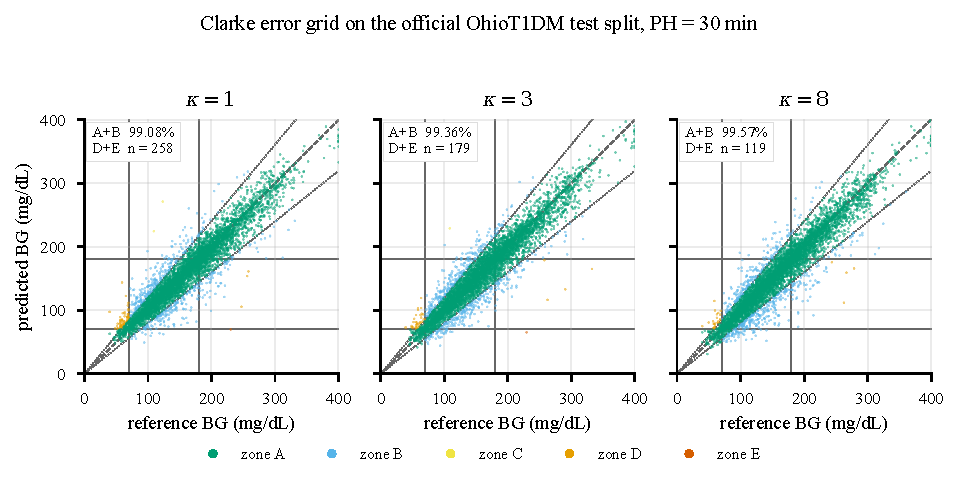
\includegraphics[width=\textwidth]{fig3_clarke_parkes_grids.pdf}
  \caption{Clarke error grid on the official OhioT1DM test split,
  $\PH = 30$~min, at three values of the asymmetry $\kappa$. Points migrate out
  of the dangerous lower-right region as $\kappa$ rises; zone percentages are
  computed on the full test set, not the plotted subsample.}
  \label{fig:clarke}
\end{figure*}

Figure~\ref{fig:clarke} shows the mechanism directly. The dangerous region for a
warning system is the lower-right (reference hypoglycemic, prediction normal),
and raising $\kappa$ empties it at the cost of a slight downward shift
elsewhere.

\subsection{Ablation C: Which Auxiliary Inputs Carry the Fusion Gain?}
\label{sec:ablation_c}

\begin{table*}[t]
\centering
\small
\setlength{\tabcolsep}{4pt}
\caption{Ablation C, condensed: every auxiliary arm as a change from its \emph{own} cohort's CGM-only control, which is the only comparison the design supports -- the 2018 and 2020 releases carry disjoint sensors, so the two blocks are not comparable to each other. Negative $\Delta$RMSE and positive $\Delta$PR-AUC are improvements. Each arm is one seed on six subjects, so the deltas are directions, not resolved effects: treatment inputs lower RMSE in both cohorts and at both horizons, and wearable streams do not do so consistently. Per-cohort tables with every metric are in the artefact directory. All ablation arms share one budget (20 epochs, fit split subsampled $2\times$), lighter than Table~\ref{tab:sota_ph30}'s (30 epochs, full fit split); rows here compare to each other, not to Table~\ref{tab:sota_ph30}.}
\label{tab:ablation_c_modality_summary}
\resizebox{\ifdim\width>\linewidth\linewidth\else\width\fi}{!}{%
\begin{tabular}{lrrrrr}
\toprule
Arm & $\Delta$RMSE 30 & $\Delta$PR-AUC 30 & $\Delta$RMSE 60 & $\Delta$PR-AUC 60 & $n$ subj \\
\midrule
2018: CGM + HR & +0.25 & -0.009 & +0.52 & -0.011 & 6 \\
2018: CGM + GSR & +0.19 & -0.022 & +0.61 & -0.023 & 6 \\
2018: CGM + steps & -0.06 & +0.008 & -0.44 & +0.008 & 6 \\
2018: CGM + treatment & -0.35 & -0.007 & -0.71 & +0.003 & 6 \\
2018: CGM + all auxiliary (incl. treatment) & -0.28 & +0.022 & -0.43 & +0.017 & 6 \\
2020: CGM + accel & -0.02 & -0.012 & +0.10 & +0.000 & 6 \\
2020: CGM + GSR & -0.09 & -0.014 & +0.05 & -0.003 & 6 \\
2020: CGM + treatment & -1.02 & +0.004 & -2.24 & -0.002 & 6 \\
2020: CGM + all auxiliary (incl. treatment) & -0.94 & -0.001 & -2.11 & +0.001 & 6 \\
\bottomrule
\end{tabular}}
\end{table*}


This study asks which auxiliary inputs carry the fusion gain. The two cohorts
wore devices with disjoint sensor sets, so an arm requiring heart rate is
measurable only on the 2018 subjects and one requiring acceleration only on
2020. Each cohort therefore gets its own CGM-only control drawn from the same six
subjects, and we do not rank across cohorts. Every arm is one seed on six
subjects, so individual deltas are directions, not resolved effects.

Wearable streams alone show no consistent benefit. At $\PH = 30$ their effects
are small, are not consistent in sign across cohorts, and
several are unfavourable: heart rate and GSR are worse than the CGM-only control
on 2018 at both horizons. The exception is steps on 2018 at $\PH = 60$, which
lowers RMSE; with one seed on six subjects we read it as a direction to re-test,
not as an effect. Treatment inputs are different. Adding insulin and carbohydrate
channels alone lowers RMSE in both cohorts and at both horizons
($\NumAblCTreatTwentyRMSEHThirty$ and $\NumAblCTreatEighteenRMSEHThirty$~mg/dL at
30~min; $\NumAblCTreatTwentyRMSEHSixty$ and $\NumAblCTreatEighteenRMSEHSixty$ at
60~min), and on RMSE the arm with every auxiliary channel, which includes them, does no
better than treatment alone. The multi-seed fusion gain of
Section~\ref{sec:results} is therefore attributable to treatment inputs. The
per-cohort tables carrying every metric are released with the artefacts.

The fusion trunk adds a \emph{gated residual} to the CGM path
(Equation~\ref{eq:fusion}), so with no auxiliary data the fusion term is exactly
zero. A unit test asserts that the multimodal forward pass reproduces the
CGM-only pass \emph{exactly} when the auxiliary channels are masked. That test is
what caught two defects that left every accuracy metric plausible: a
normalisation placed on the summed representation, and auxiliary validity read
from a single sensor's mask. A third defect of the same kind survived it and was
found only after submission: the per-window presence flag ignored treatment
channels, which have no observation mask, so insulin and carbohydrate inputs
could not enable the fusion branch (Appendix~\ref{sec:metabonet}). The results
here are from the corrected code.

The identity above is architectural, not a performance bound: the CGM path is
trained jointly with the fusion path, and several wearable arms land below their
control at the point estimate.

\subsection{Leakage Ladder at Sixty Minutes}
\label{sec:appendix_ablation_d}

\begin{table*}[t]
\centering
\small
\setlength{\tabcolsep}{4pt}
\caption{Ablation D: what lookahead bias buys (PH = 60 min). Arms are \emph{not} scored on the same test set: changing the split is the flaw being measured. All ablation arms share one budget (20 epochs, fit split subsampled $2\times$), lighter than Table~\ref{tab:sota_ph30}'s (30 epochs, full fit split); rows here compare to each other, not to Table~\ref{tab:sota_ph30}.}
\label{tab:ablation_d_leakage_ph60}
\resizebox{\ifdim\width>\linewidth\linewidth\else\width\fi}{!}{%
\begin{tabular}{lrrrrrrr}
\toprule
Arm & RMSE & MAE & PR-AUC & Se@5\% & A+B (\%) & Lag (min) & $n$ test \\
\midrule
Strict causal pipeline (ours) & 31.61 & 22.63 & 0.772 & 0.849 & 97.80 & 40.0 & 28335 \\
+ unembargoed random split & 30.07 & 21.34 & 0.811 & 0.846 & 98.01 & -- & 29932 \\
+ full-series interpolation \& centred features & 27.11 & 18.30 & 0.867 & 0.895 & 98.35 & -- & 37704 \\
\bottomrule
\end{tabular}}
\end{table*}


Table~\ref{tab:ablation_d_leakage_ph60} repeats the ladder of
Table~\ref{tab:ablation_d_leakage_ph30} at $\PH = 60$~min. The feature and label
flaws inflate apparent performance at both horizons (measured RMSE lower and
PR-AUC higher than under the strict pipeline), so that inflation is not an
artefact of the thirty-minute horizon. The split behaves differently: on its own
it leaves measured RMSE $\NumLeakSplitRMSEIncreasePct\%$ higher than under the
strict pipeline at $\PH = 30$ but $\NumLeakSplitRMSEReductionPctHSixty\%$
lower at $\PH = 60$ (PR-AUC higher by $\NumLeakSplitPRAUCIncreaseHSixty$),
so its cost is horizon-dependent and is not negligible at the longer horizon.
The arms are scored on different test sets, which limits how finely these
differences can be read.

\paragraph{A methodological caution.}
We made this mistake ourselves. Our first control computed centred statistics
\emph{per window}, on a slice that ends at the anchor. In other words, the
centring had no future to reach into, the ``leaky'' arm leaked nothing, and the
study reported an inflation near zero. We caught it only because that null result
was implausible. The realistic mistake is to compute
features on the whole frame and slice afterwards; the order of operations
\emph{is} the flaw, and a leakage study that gets it wrong reports a reassuring
zero. A mutation test that corrupts the future and requires the control arm's
inputs to \emph{move} is what makes the measurement trustworthy, and it is the
first thing we would ask of any such study.

\subsection{Ablation E: Does the Soft-Label Boundary Band Matter?}
\label{sec:ablation-e}

\begin{table*}[t]
\centering
\small
\setlength{\tabcolsep}{4pt}
\caption{Ablation E: the soft-label boundary band (PH = 30 min). The band column is each arm's \emph{realised} band. The estimated arm derives it from the fold's MARD against paired capillary reference BG; a band below the device specification falls back to the specification, and \texttt{soft\_label.band\_source} in the JSON records which happened. All ablation arms share one budget (20 epochs, fit split subsampled $2\times$), lighter than Table~\ref{tab:sota_ph30}'s (30 epochs, full fit split); rows here compare to each other, not to Table~\ref{tab:sota_ph30}.}
\label{tab:ablation_e_soft_label_ph30}
\resizebox{\ifdim\width>\linewidth\linewidth\else\width\fi}{!}{%
\begin{tabular}{lrrrrrrrr}
\toprule
Arm & Band (mg/dL) & PR-AUC & ROC-AUC & Se@5\% & FAPD@5\% & Onset lead (min) & RMSE & A+B (\%) \\
\midrule
Hard labels & -- & 0.850 & 0.9899 & \textbf{0.962} & 3.05 & \textbf{26.9} & 18.50 & 99.34 \\
Fixed $\pm$5 mg/dL & 5.00 & \textbf{0.865} & 0.9911 & 0.960 & 2.98 & 26.9 & 18.54 & 99.39 \\
Fixed $\pm$10 mg/dL & 10.00 & 0.865 & \textbf{0.9912} & 0.959 & 2.87 & 26.4 & 18.49 & 99.36 \\
Fixed $\pm$20 mg/dL & 20.00 & 0.854 & 0.9899 & 0.955 & 2.50 & 26.2 & \textbf{18.42} & 99.38 \\
Estimated (MARD) & 7.24 & 0.864 & 0.9909 & 0.957 & 2.84 & 26.7 & 18.49 & \textbf{99.40} \\
\bottomrule
\end{tabular}}
\end{table*}

\begin{table*}[t]
\centering
\small
\setlength{\tabcolsep}{4pt}
\caption{Ablation E: the soft-label boundary band (PH = 60 min). The band column is each arm's \emph{realised} band. The estimated arm derives it from the fold's MARD against paired capillary reference BG; a band below the device specification falls back to the specification, and \texttt{soft\_label.band\_source} in the JSON records which happened. All ablation arms share one budget (20 epochs, fit split subsampled $2\times$), lighter than Table~\ref{tab:sota_ph30}'s (30 epochs, full fit split); rows here compare to each other, not to Table~\ref{tab:sota_ph30}.}
\label{tab:ablation_e_soft_label_ph60}
\resizebox{\ifdim\width>\linewidth\linewidth\else\width\fi}{!}{%
\begin{tabular}{lrrrrrrrr}
\toprule
Arm & Band (mg/dL) & PR-AUC & ROC-AUC & Se@5\% & FAPD@5\% & Onset lead (min) & RMSE & A+B (\%) \\
\midrule
Hard labels & -- & 0.761 & 0.9687 & 0.835 & 3.69 & 43.7 & 31.61 & 97.78 \\
Fixed $\pm$5 mg/dL & 5.00 & 0.777 & 0.9713 & \textbf{0.856} & 3.59 & \textbf{44.4} & 31.64 & 97.87 \\
Fixed $\pm$10 mg/dL & 10.00 & 0.772 & 0.9714 & 0.849 & 3.37 & 43.5 & 31.61 & 97.80 \\
Fixed $\pm$20 mg/dL & 20.00 & 0.762 & 0.9697 & 0.838 & 2.87 & 42.5 & \textbf{31.48} & 97.84 \\
Estimated (MARD) & 7.24 & \textbf{0.782} & \textbf{0.9716} & 0.847 & 3.26 & 43.7 & 31.55 & \textbf{97.89} \\
\bottomrule
\end{tabular}}
\end{table*}


Soft labels at the hypoglycemia boundary are due to \citet{fang2026glucose}; what
follows sweeps our own formulation of the band, not a reproduction of theirs.
Their soft label is a risk-probability mapping rather than a band, so these
results neither confirm nor contradict theirs; their own ablation reports soft
labels improving sensitivity and AUC over hard thresholds. We
sweep it from a hard indicator through three pinned widths to a band derived from
the fold's estimated measurement error. The estimate is a
MARD against the paired capillary reference readings released alongside the CGM
stream ($\NumAblEMardPairs$ pairs over the twelve subjects, $\NumAblEMardPct\%$,
giving a $\pm\NumAblEMardBand$~mg/dL band); a noise estimate taken from the CGM
signal itself recovers an order of magnitude less, because the released stream
has already been smoothed, and is not usable for this purpose.

No configuration dominates. PR-AUC spans $\NumAblEPRAUCSpreadHThirty$ across all
five arms at $\PH = 30$ and $\NumAblEPRAUCSpreadHSixty$ at $\PH = 60$, and the
band width does not order the results: the estimated $\pm\NumAblEMardBand$~mg/dL
band performs like the pinned widths on either side of it. With one seed per arm
we do not read differences of this size as separating the arms, and we do not
nominate a winner. The one direction that is consistent across both horizons is
the alarm rate: hard labels give the highest false-alarm rate per day at
$\PH = 30$ ($\NumAblEHardFAPDHThirty$ against $\NumAblEFAPDMinHThirty$) and at
$\PH = 60$ ($\NumAblEHardFAPDHSixty$ against $\NumAblEFAPDMinHSixty$), and every
soft band lowers it. This is the direction the mechanism predicts, since a
network not required to fit device noise within a reading of the threshold
should raise fewer boundary-crossing alarms.

The practical reading is that the band is a low-sensitivity knob, and that is
what justifies the configuration we ship: a pinned $\pm 10$~mg/dL band rather
than an estimated one, because the estimate buys nothing measurable here and a
pinned width is reproducible on cohorts that release no paired reference
readings, which is most of them. The estimator earns its place by making the
mode ablatable at all rather than by winning: derived from the CGM signal alone
the band collapses below the display resolution of the device, and this table's
treatment arm would have been an unintended copy of its control.

Every ablation in this appendix shares one budget ($\NumAblADEpochs$ epochs, fit
split subsampled $2\times$), so the tables are comparable to one another; none is
comparable to the benchmark of Table~\ref{tab:sota_ph30}, which is trained at 30
epochs on the full fit split.
